% -*- TeX:Rnw:si -*-
% ----------------------------------------------------------------
% .R Sweave file  ************************************************
% ----------------------------------------------------------------
%%
%\documentclass[a4paper,12pt,english]{article}
\documentclass[a4paper,12pt,slovene]{article}
\usepackage{babel}
\input{abpkg}
\input{abcmd}
\input{abpage}
\usepackage{pgf,pgfarrows,pgfnodes,pgfautomata,pgfheaps,pgfshade}
\usepackage{amsmath,amssymb}
\usepackage{colortbl}
\usepackage{Sweave}
\input{mysweave}
\usepackage{lmodern}
\input{abfont}
%\SweaveOpts{keep.source=true}
%\setkeys{Gin}{width=0.8\textwidth} % set graphicx parameter
% ----------------------------------------------------------------
\begin{document}
%% Sweave settings for includegraphics default plot size (Sweave default is 0.8)
%% notice this must be after begin{document}
%%% \setkeys{Gin}{width=0.9\textwidth}
% ----------------------------------------------------------------
\title{\R in multivariatna normalna porazdelitev}
\author{A. Blejec}
%\address{}%
%\email{}%
%
%\thanks{}%
%\subjclass{}%
%\keywords{}%

%\date{}%
%\dedicatory{}%
%\commby{}%
\maketitle
% ----------------------------------------------------------------
\begin{abstract}
Opisanih je nekaj primerov za uporabo funkcij v zvezi z  multivariatno normalno porazdelitvijo.
\end{abstract}
% ----------------------------------------------------------------


\section{Paket \pkg{mvtnorm}}

Paket \pkg{mvtnorm} vsebuje funkcije, s katerimi lahko obvladamo osnovne �tiri naloge v zvezi z multivariatno normalno on multivariatno $t$ porazdelitvijo.

\begin{Schunk}
\begin{Sinput}
> library(mvtnorm)
\end{Sinput}
\end{Schunk}

\subsection{Bivariatna normalna porazdelitev}

\begin{Schunk}
\begin{Sinput}
> n <- 2
> dx <- 0.2
> mu <- rep(0, n)
> sigma <- diag(n)
> sigma <- matrix(c(1, -0.3, -0.3, 4), ncol = n)
> x1 <- seq(-5, 5, dx)
> x2 <- seq(-5, 5, dx)
> x <- expand.grid(x1 = x1, x2 = x2)
> z <- matrix(dmvnorm(x, mu, sigma), nrow = length(x1), 
+     ncol = length(x2))
> for (i in seq(-30, 30, 5)) persp(x1, x2, z, phi = 30, 
+     theta = i)
\end{Sinput}
\end{Schunk}
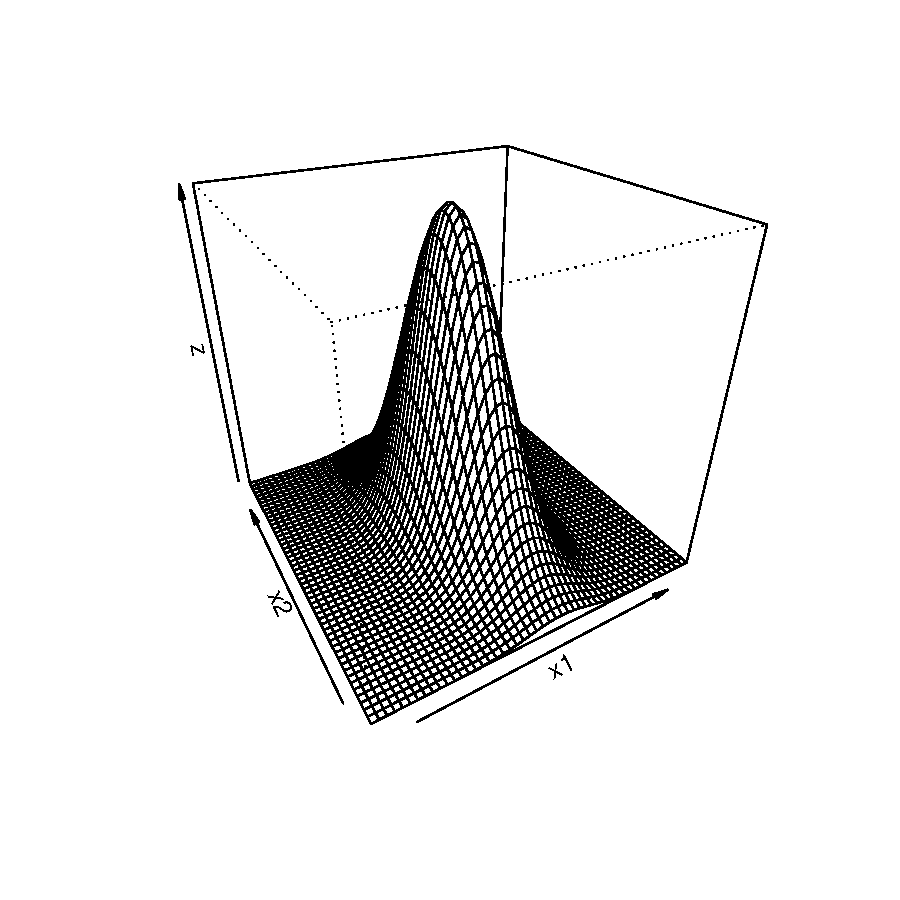
\includegraphics{mvtnorm-003}

\begin{Schunk}
\begin{Sinput}
> dx = 0.53321
> x1 <- seq(-5, 5, dx)
> x2 <- seq(-5, 5, dx)
> X <- expand.grid(x = x1, y = x2)
> z = with(X, matrix(1/(x^2 + y^2), nrow = length(x1), 
+     ncol = length(x2)))
> persp(x1, x2, z, phi = 30, theta = 45, col = "lightblue", 
+     shade = 1)
\end{Sinput}
\end{Schunk}
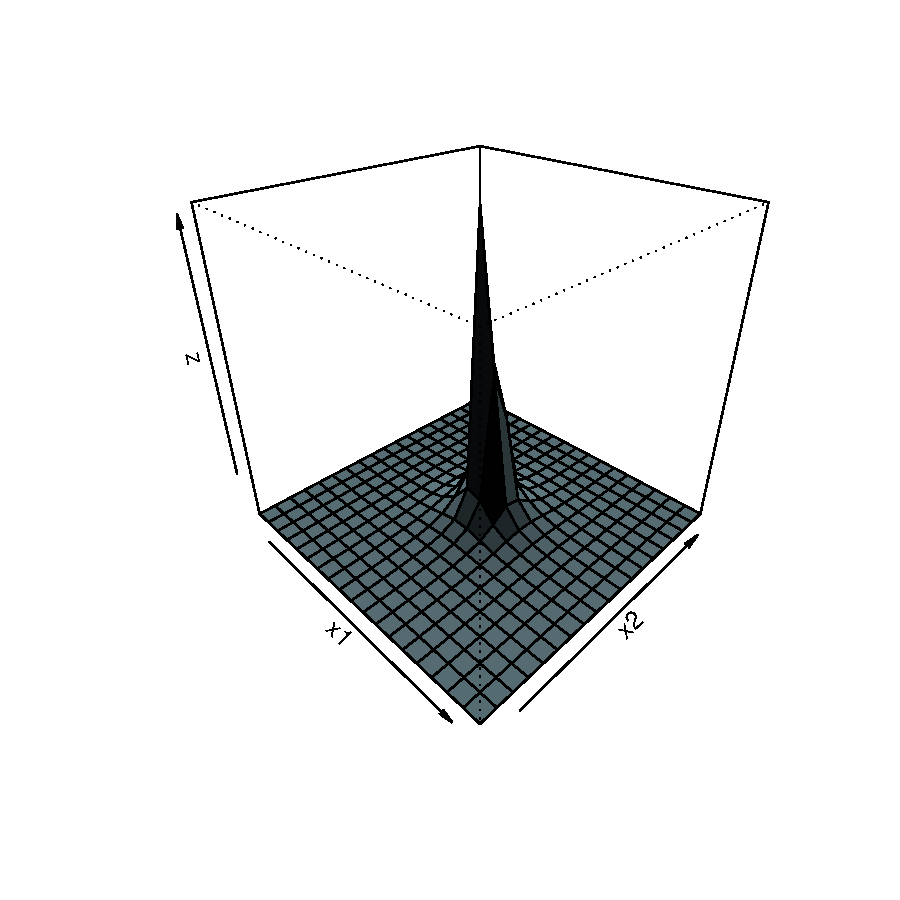
\includegraphics{mvtnorm-004}

\begin{Schunk}
\begin{Sinput}
> dx = 0.53
> x1 <- seq(-5, 5, dx)
> x2 <- seq(-5, 5, dx)
> X <- expand.grid(x = x1, y = x2)
> z = with(X, matrix(x^3 + y^2, nrow = length(x1), ncol = length(x2)))
> contour(x1, x2, z)
\end{Sinput}
\end{Schunk}
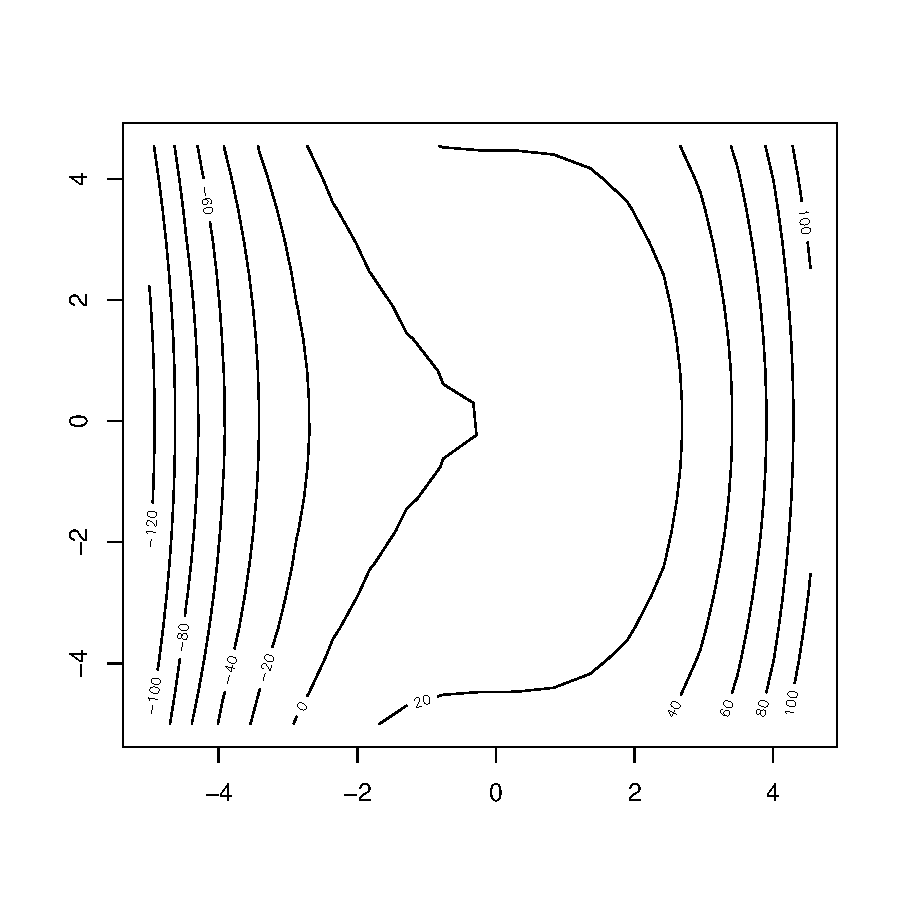
\includegraphics{mvtnorm-005}

\begin{Schunk}
\begin{Sinput}
> persp(x1, x2, z, phi = 30, theta = 340, col = "lightblue", 
+     shade = 1)
\end{Sinput}
\end{Schunk}
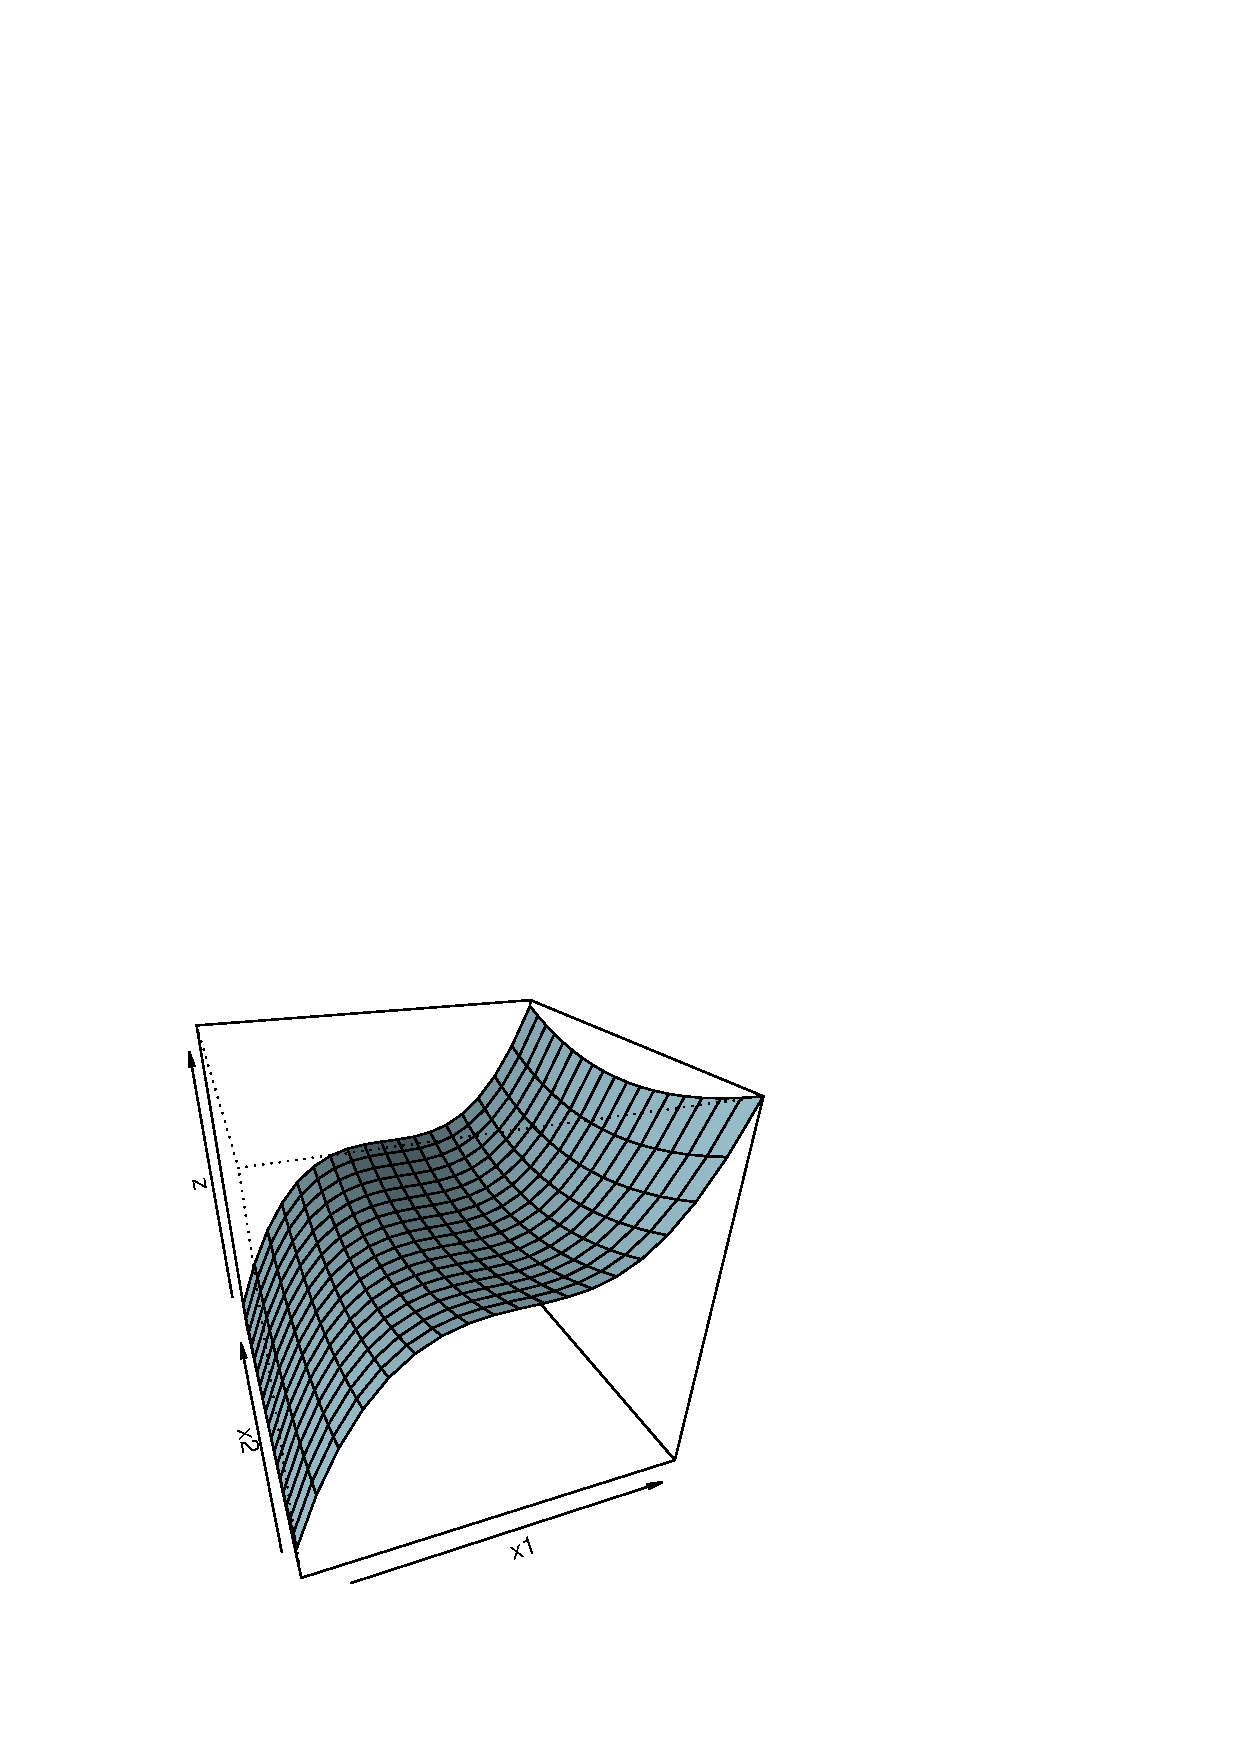
\includegraphics{mvtnorm-006}

\begin{Schunk}
\begin{Sinput}
> library(fields)
\end{Sinput}
\begin{Soutput}
Package 'spam' is loaded.  Version0.13-2 (2008-01-04).

Type demo( spam) for some demos,
 help( Spam) for an overview of this package.

 Try help(fields) for an overview of this library 
\end{Soutput}
\end{Schunk}


\clearpage
\begin{Schunk}
\begin{Sinput}
> dx = 1
> x1 <- seq(200, 600, dx)
> x2 <- seq(200, 600, dx)
> X <- expand.grid(x = x1, y = x2)
> pari <- with(X, which((x^2 - y^2) == 2008))
> pari <- X[pari, ]
> z <- with(X, matrix(x^2 - y^2, nrow = length(x1), ncol = length(x2)))
> contour(x1, x2, z)
> points(pari, col = "red", pch = 16)
\end{Sinput}
\end{Schunk}
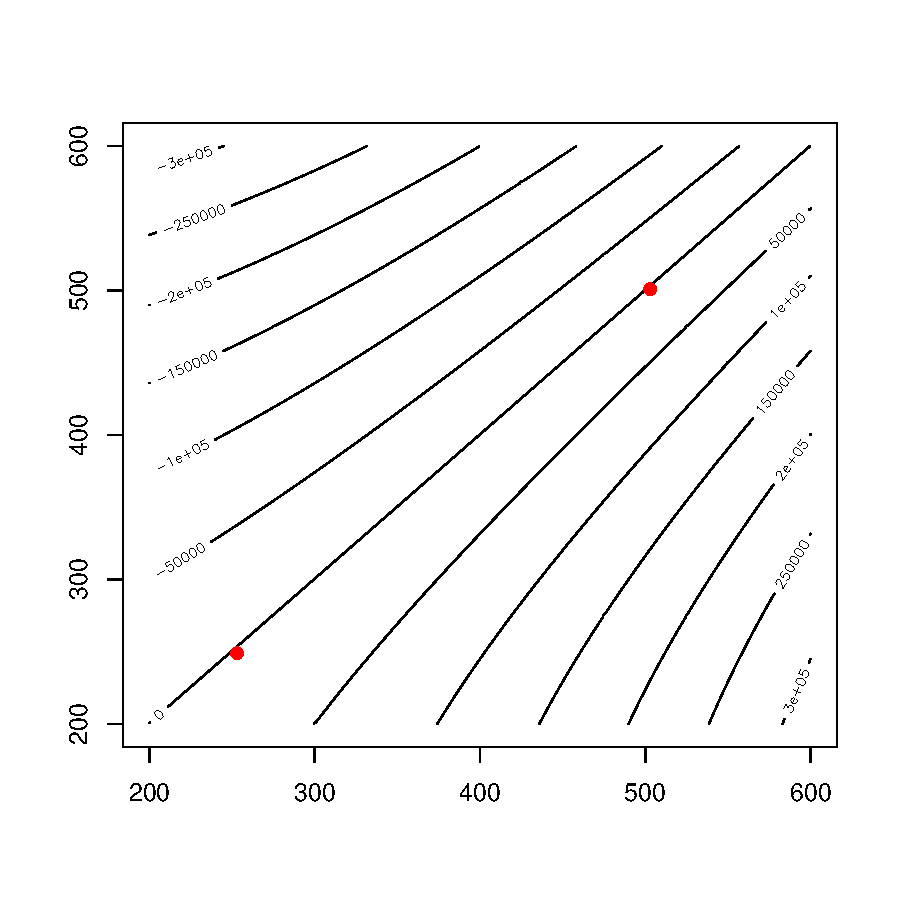
\includegraphics{mvtnorm-008}

\begin{Schunk}
\begin{Sinput}
> dx = 20
> x1 <- seq(200, 600, dx)
> x2 <- seq(200, 600, dx)
> X <- expand.grid(x = x1, y = x2)
> z <- with(X, matrix(x^2 - y^2, nrow = length(x1), ncol = length(x2)))
> pm <- drape.plot(x1, x2, z, phi = 30, theta = -60, shade = 0.1, 
+     col = terrain.colors(128))
> pushpin(pari[, 1], pari[, 2], 2008, pm, text = apply(pari, 
+     1, paste, collapse = " , "), col = "red", height = 0.1, 
+     cex = 1)
\end{Sinput}
\end{Schunk}
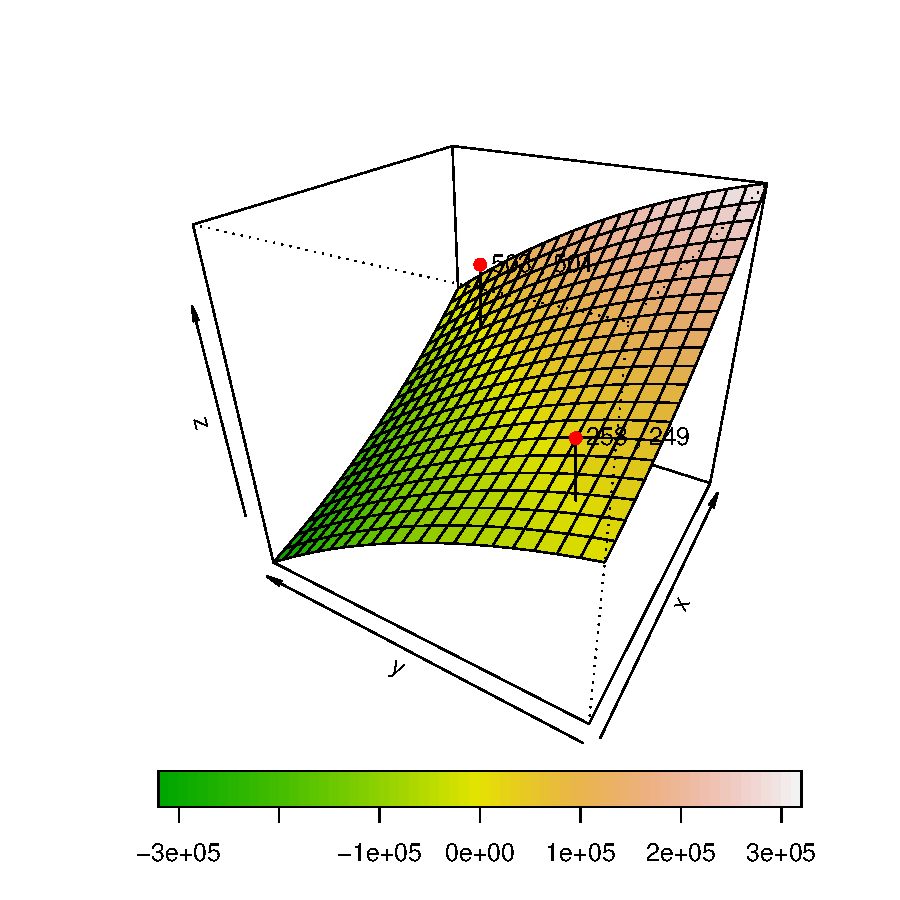
\includegraphics{mvtnorm-009}


% ----------------------------------------------------------------
%\bibliographystyle{amsplain}
%\bibliography{}
\end{document}
% ----------------------------------------------------------------
